\thispagestyle{fancy}
\vspace*{40 pt}
\subsection{Tela ajustes slotter}\label{telaAjustesSlotter}
 Essa tela é acessada através do botão "\textgreater" no menu superior esquerdo da tela de ajustes da ultima impressora, pelo botão "\textless{}" no menu superior esquerdo 
 da tela ajustes perfuradora, pelo botão "SLT" em qualquer tela de ajustes e pelo botão ajustes da tela comando slotter.
 \vspace*{\fill}
 \begin{figure}[h]
  \centering
  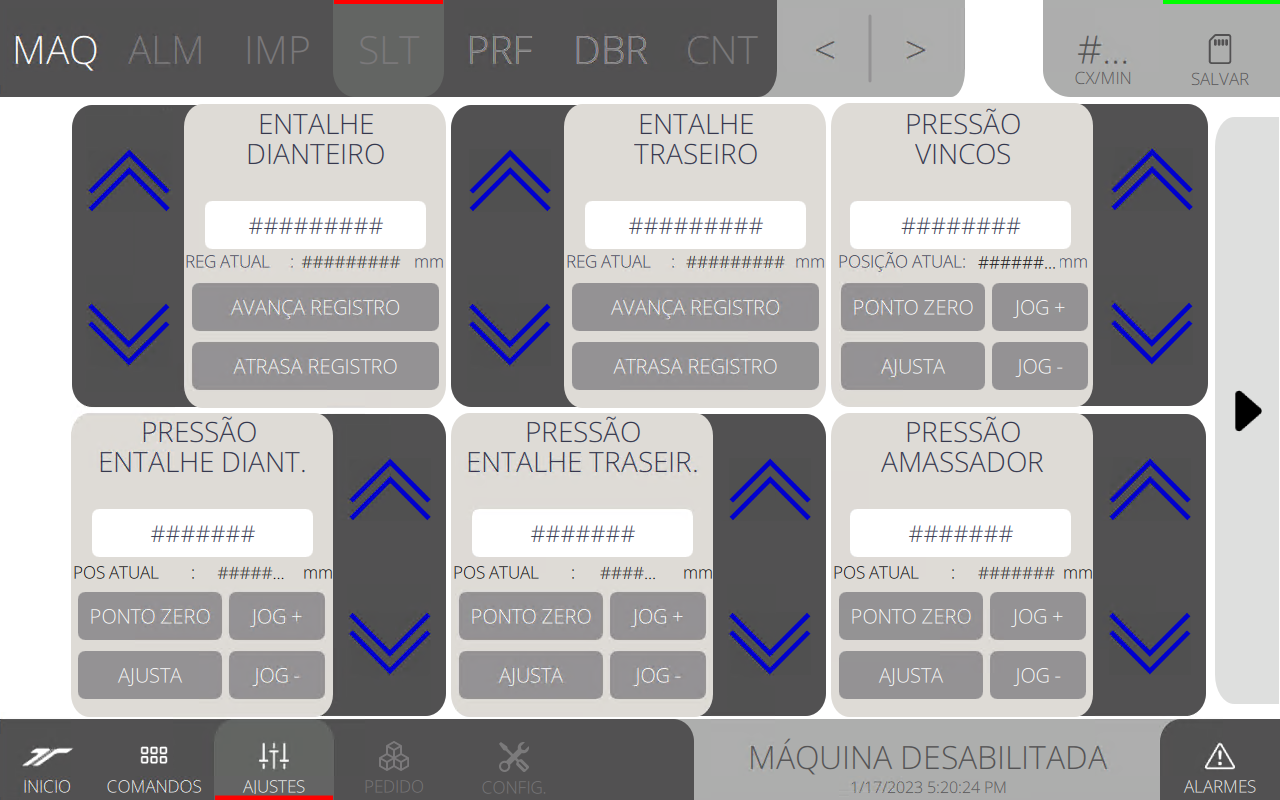
\includegraphics[width=576px,height=360px]{src/imagesFlexo/05-slotter/settings/e-Tela-Principal.png}
\end{figure}
\vspace*{\fill}

\newpage
\thispagestyle{fancy}
\vspace*{40 pt}
\subsubsection{\small{Ajuste pressão do amassador}}\label{telaAjustesSlotterAjustePressaoDoAmassador}
\vspace*{\fill}
\begin{figure}[h]
  \centering
  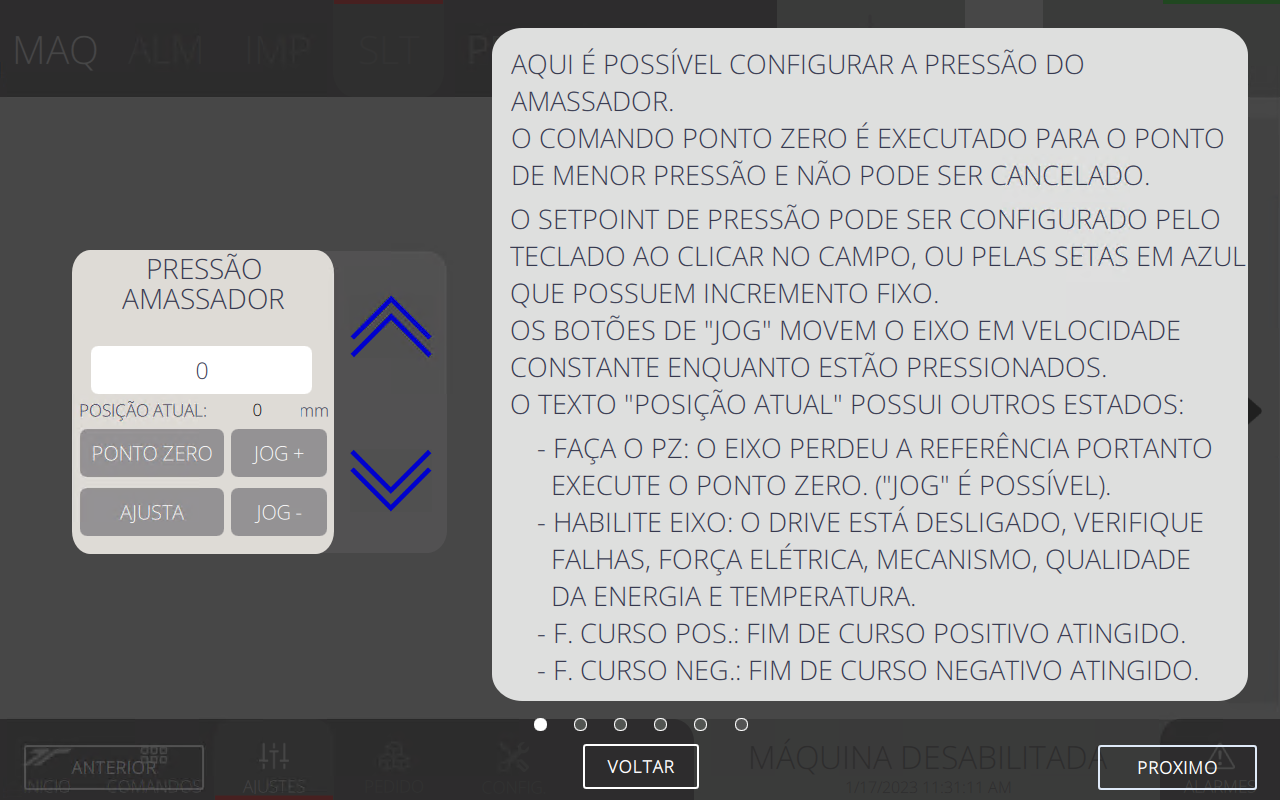
\includegraphics[width=576px,height=360px]{src/imagesFlexo/05-slotter/settings/e-1.png}
\end{figure}
\vspace*{\fill}

\newpage
\thispagestyle{fancy}
\vspace*{40 pt}
\subsubsection{\small{Ajuste pressão do entalhe traseiro}}\label{telaAjustesSlotterAjustePressaoDoEntalheTraseiro}
\vspace*{\fill}
\begin{figure}[h]
  \centering
  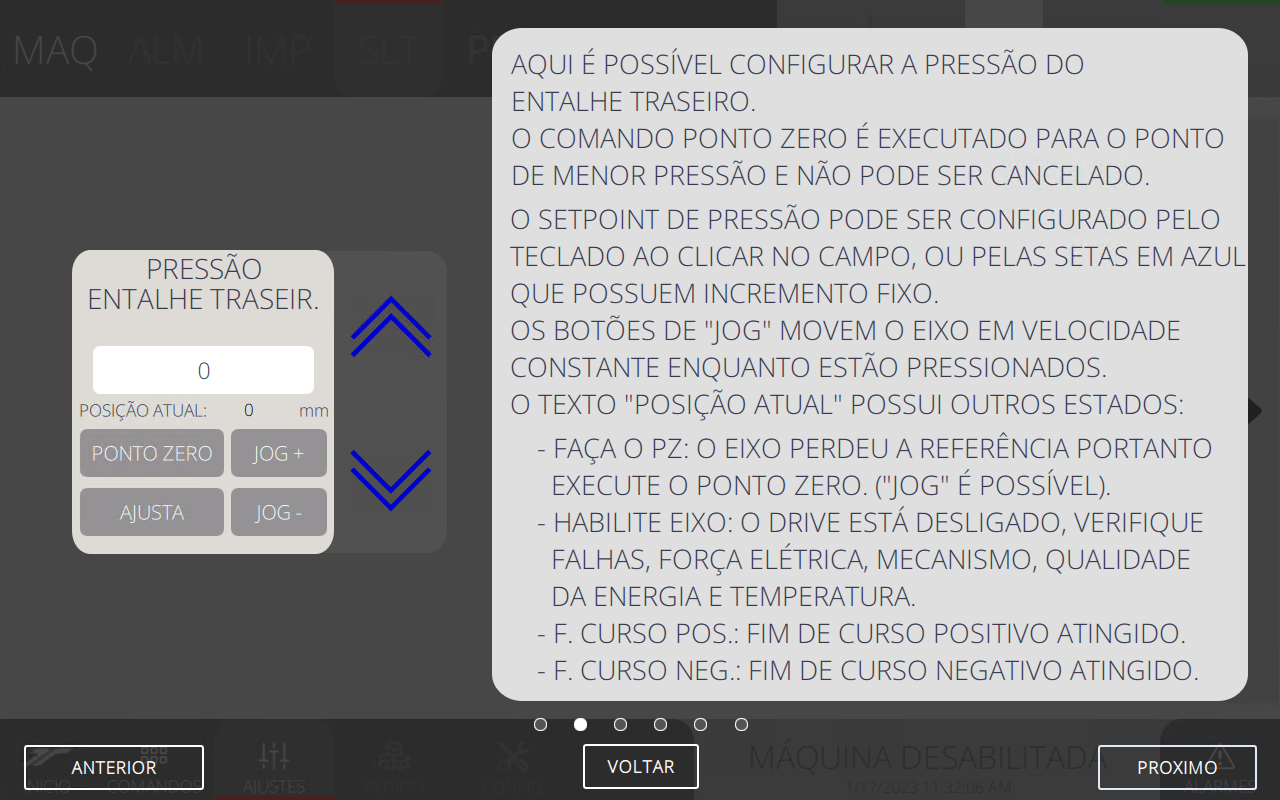
\includegraphics[width=576px,height=360px]{src/imagesFlexo/05-slotter/settings/e-2.png}
\end{figure}
\vspace*{\fill}

\newpage
\thispagestyle{fancy}
\vspace*{40 pt}
\subsubsection{\small{Ajuste pressão do entalhe dianteiro}}\label{telaAjustesSlotterAjustePressaoDoEntalheDianteiro}
\vspace*{\fill}
\begin{figure}[h]
  \centering
  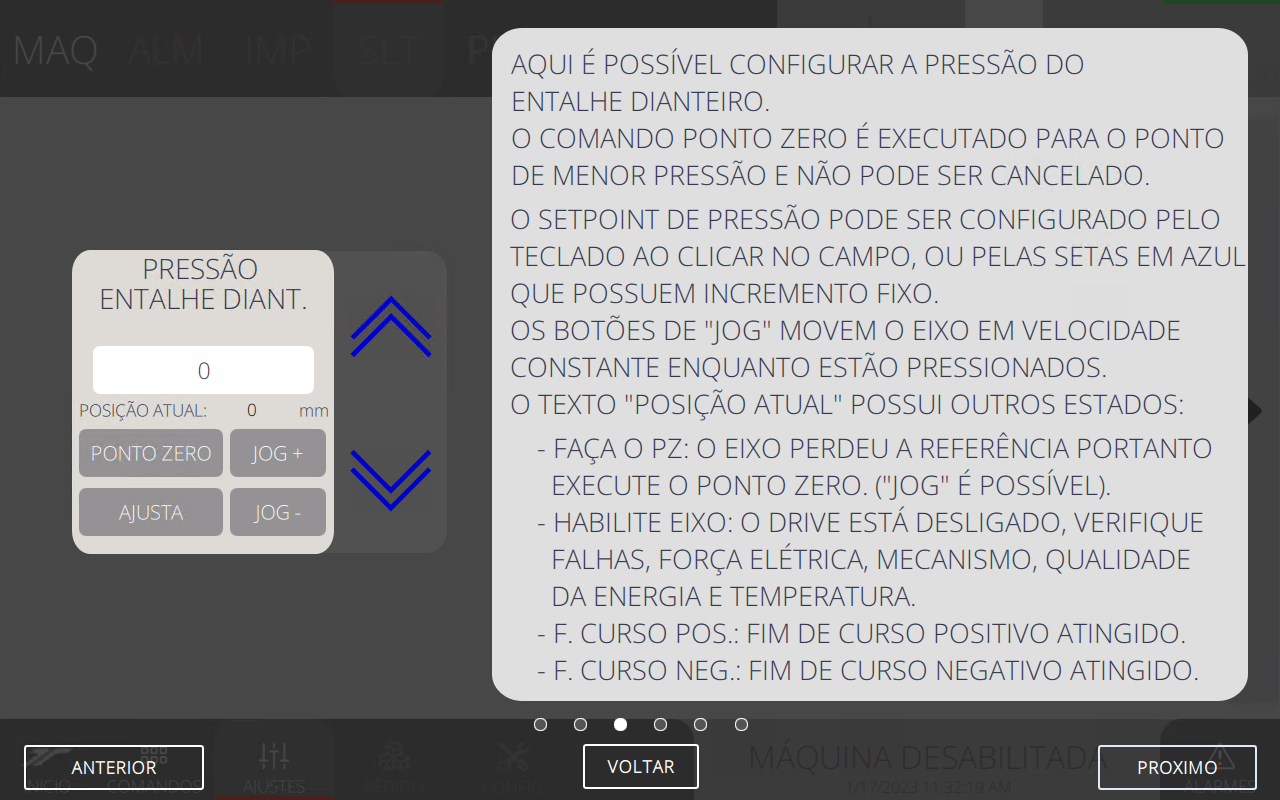
\includegraphics[width=576px,height=360px]{src/imagesFlexo/05-slotter/settings/e-3.png}
\end{figure}
\vspace*{\fill}

\newpage
\thispagestyle{fancy}
\vspace*{40 pt}
\subsubsection{\small{Ajuste pressão vincos}}\label{telaAjustesSlotterAjustePressaoVincos}
\vspace*{\fill}
\begin{figure}[h]
  \centering
  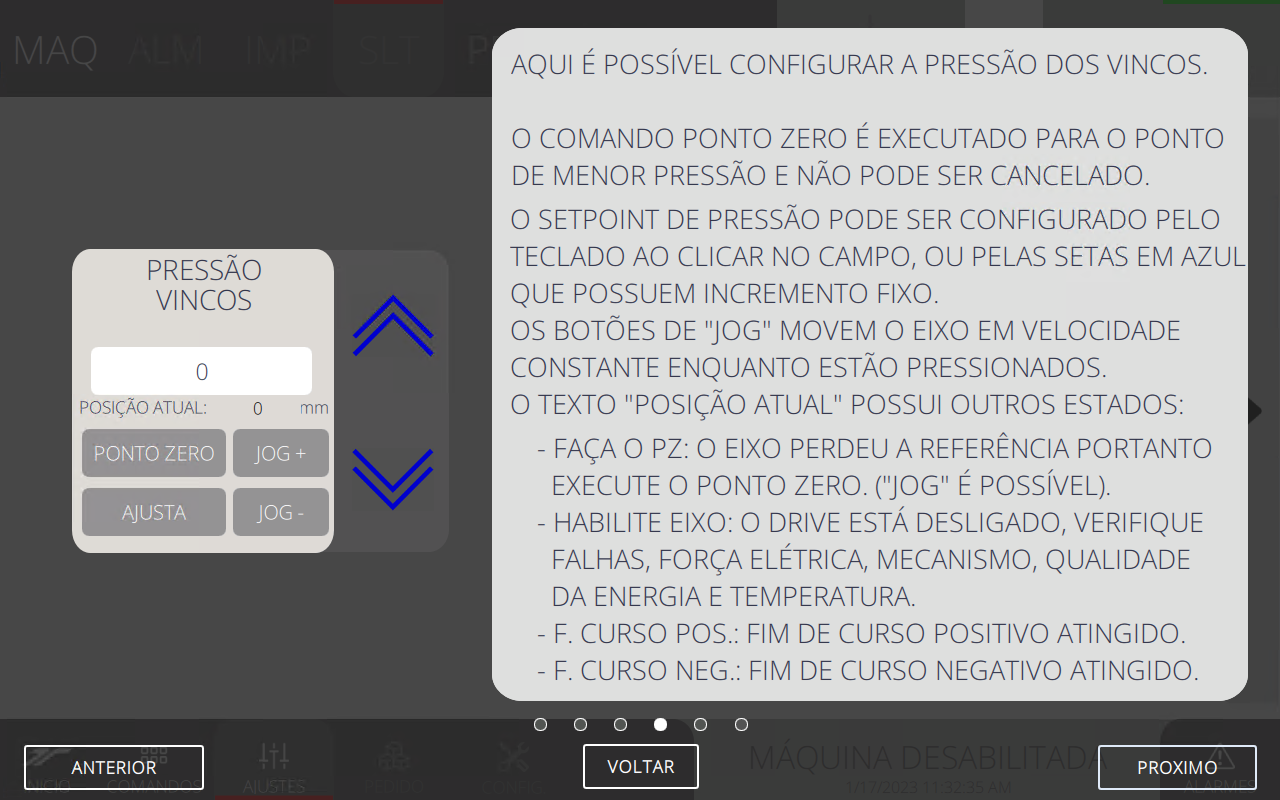
\includegraphics[width=576px,height=360px]{src/imagesFlexo/05-slotter/settings/e-4.png}
\end{figure}
\vspace*{\fill}

\newpage
\thispagestyle{fancy}
\vspace*{40 pt}
\subsubsection{\small{Ajuste registro entalhe traseiro}}\label{telaAjustesSlotterAjusteRegistroEntalheTraseiro}
\vspace*{\fill}
\begin{figure}[h]
  \centering
  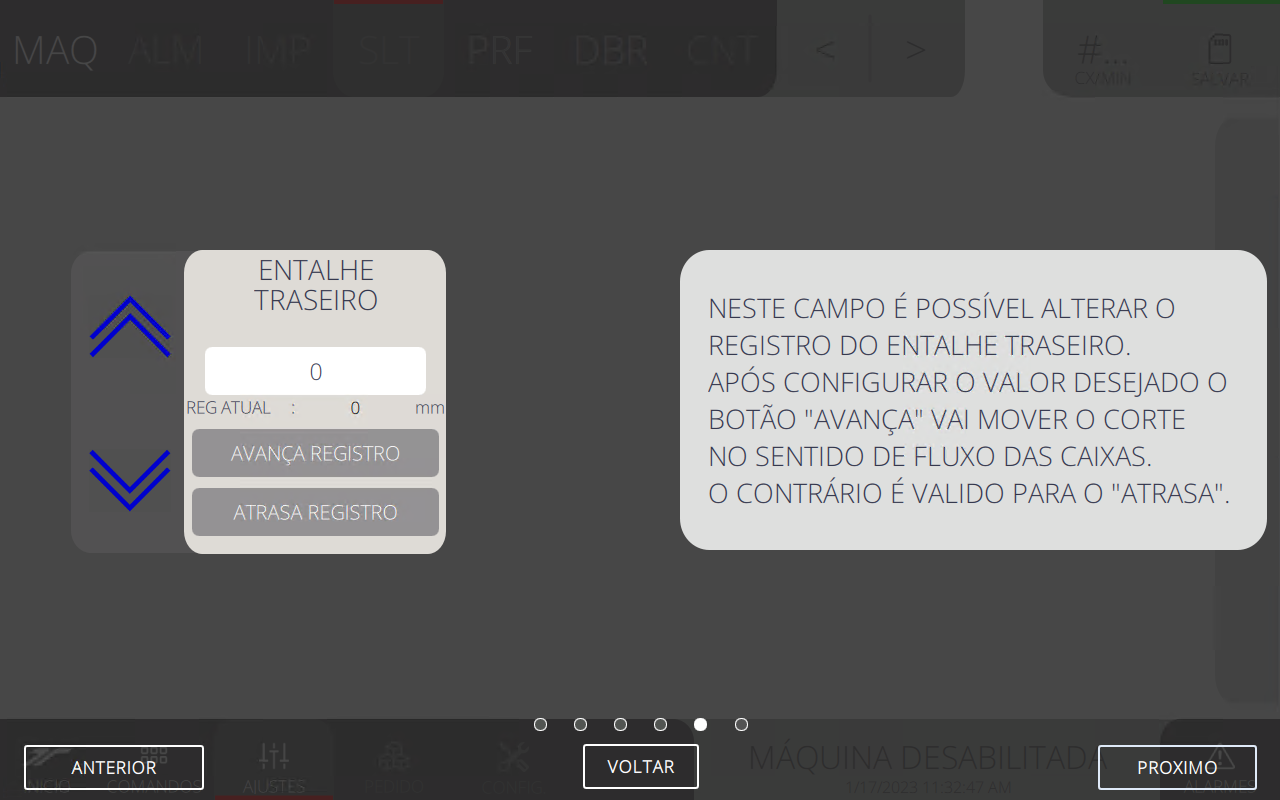
\includegraphics[width=576px,height=360px]{src/imagesFlexo/05-slotter/settings/e-5.png}
\end{figure}
\vspace*{\fill}

\newpage
\thispagestyle{fancy}
\vspace*{40 pt}
\subsubsection{\small{Ajuste registro entalhe dianteiro}}\label{telaAjustesSlotterAjusteRegistroEntalheDianteiro}
\vspace*{\fill}
\begin{figure}[h]
  \centering
  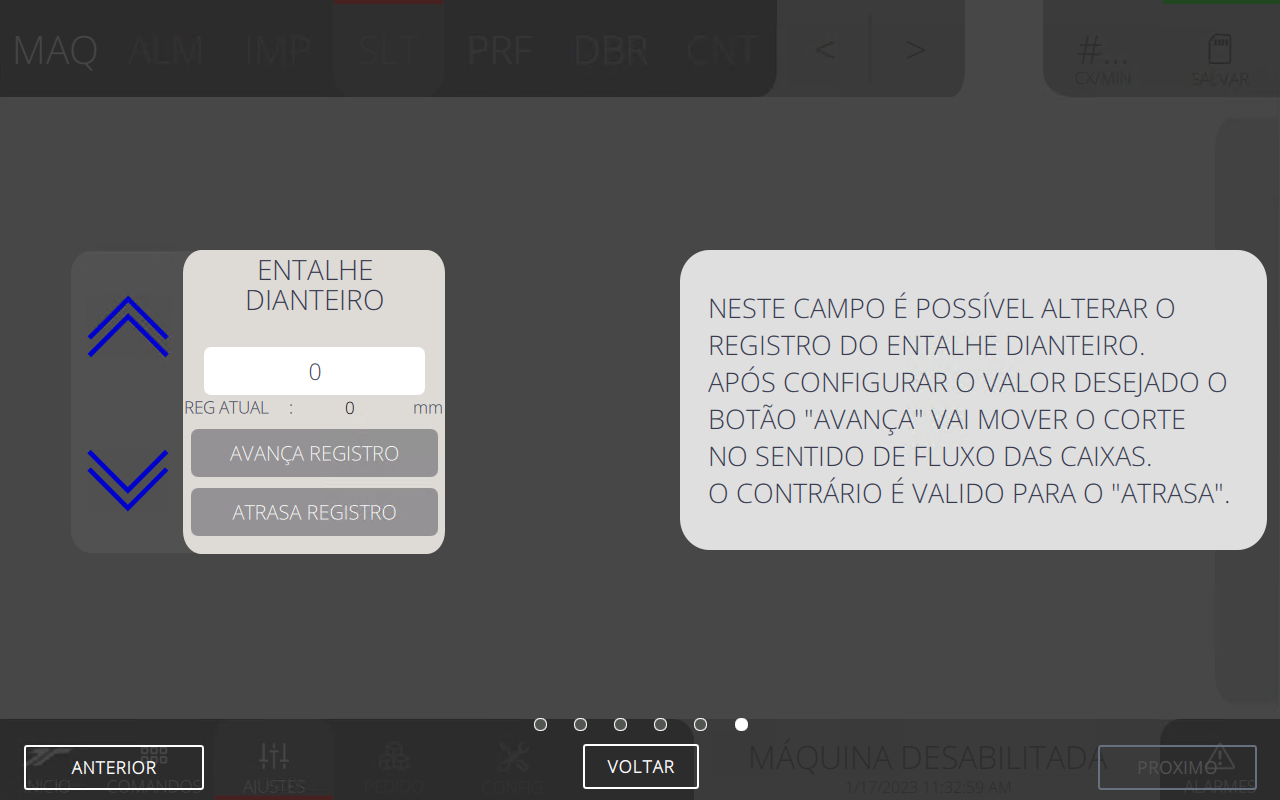
\includegraphics[width=576px,height=360px]{src/imagesFlexo/05-slotter/settings/e-6.png}
\end{figure}
\vspace*{\fill}

\newpage
\thispagestyle{fancy}
\vspace*{40 pt}
\subsection{Segunda tela ajustes slotter}\label{telaAjustesSlotter2}
Esta tela é acessada pelo botão direito "\textgreater" na tela de ajustes slotter. A lógica dos outros menus continua sendo a mesma da sua tela "pai" e para voltar a tela anterior basta clicar no botão esquerdo "\textless{}".
\vspace*{\fill}
\begin{figure}[h]
  \centering
  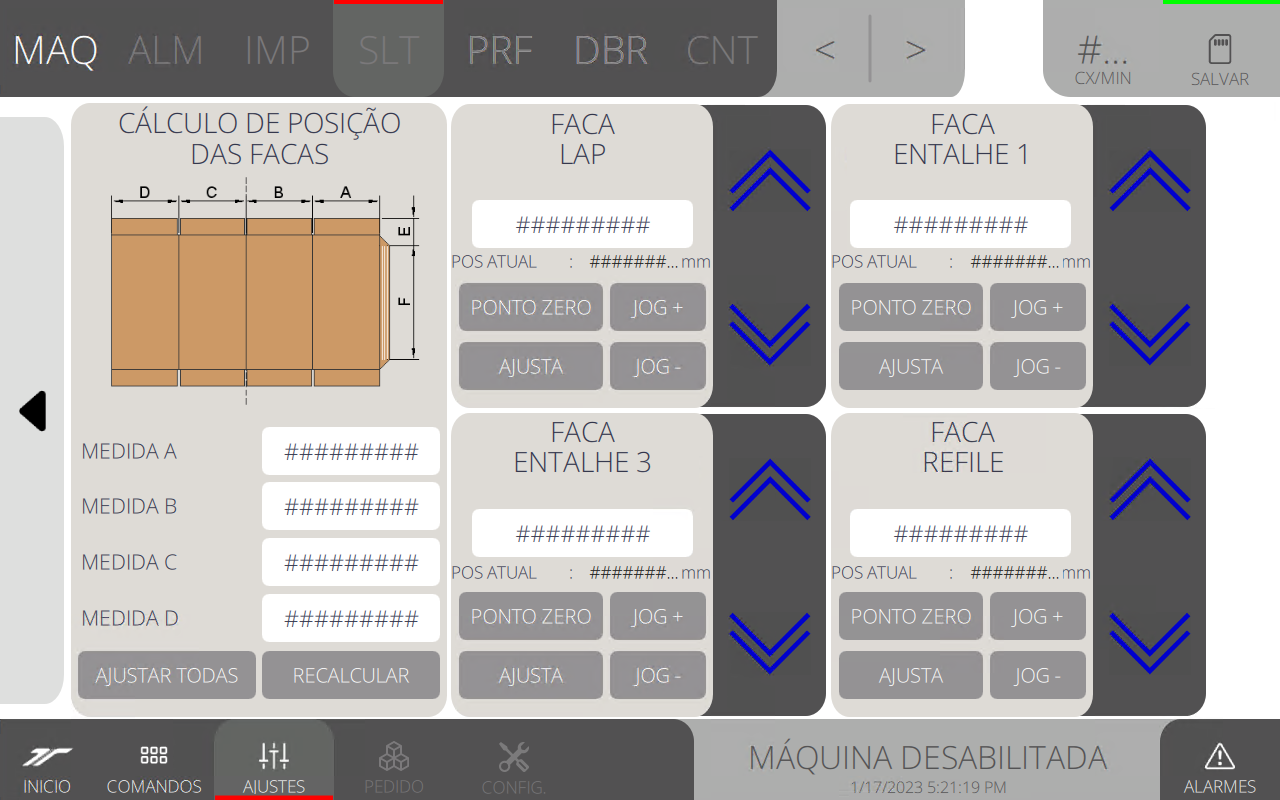
\includegraphics[width=576px,height=360px]{src/imagesFlexo/05-slotter/settings/e-Tela-Principal-2.png}
\end{figure}
\vspace*{\fill}

\newpage
\thispagestyle{fancy}
\vspace*{40 pt}
\subsubsection{\small{Cálculo da posição axial das facas}}\label{telaAjustesSlotterCalculoDaPosicaoAxialDasFacas}
\vspace*{\fill}
\begin{figure}[h]
  \centering
  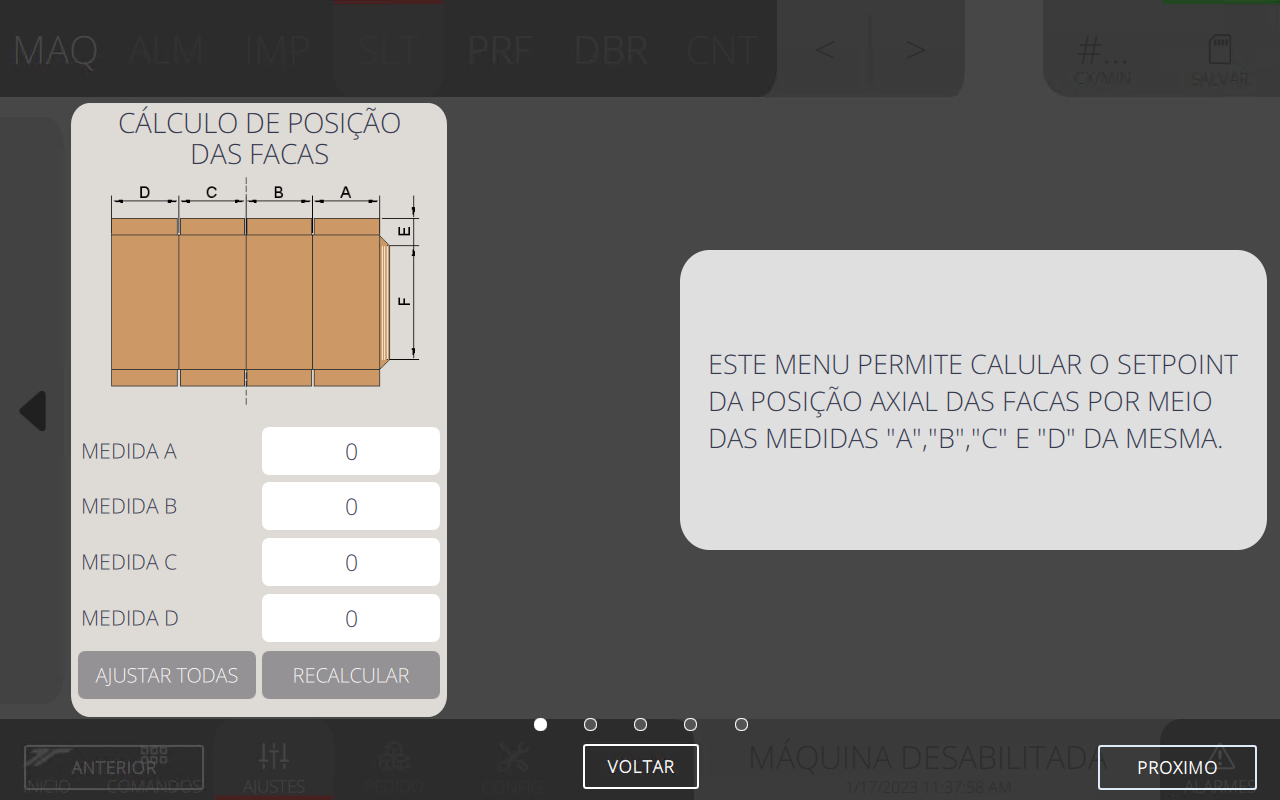
\includegraphics[width=576px,height=360px]{src/imagesFlexo/05-slotter/settings/e-7.png}
\end{figure}
\vspace*{\fill}

\newpage
\thispagestyle{fancy}
\vspace*{40 pt}
\subsubsection{\small{Ajuste da posição axial da faca LAP}}\label{telaAjustesSlotterAjusteDaPosicaoAxialDaFacaLap}
\vspace*{\fill}
\begin{figure}[h]
  \centering
  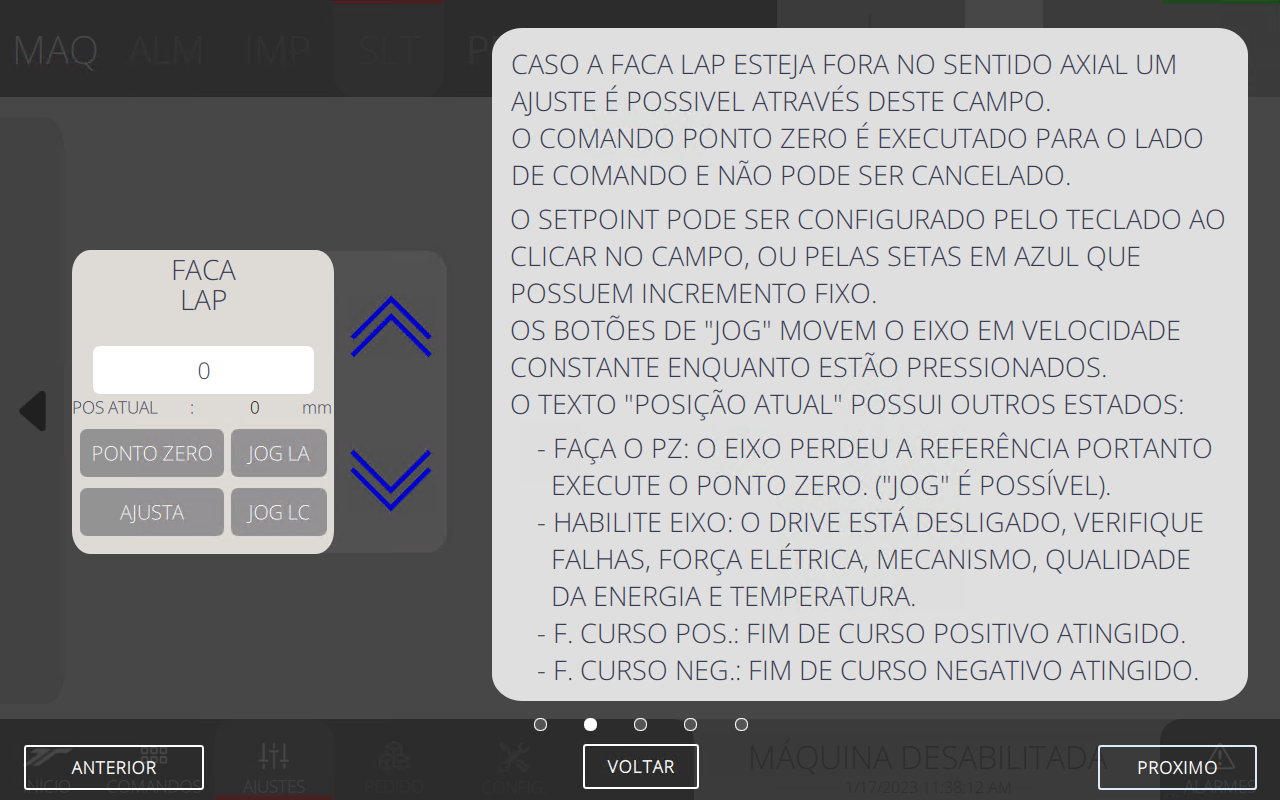
\includegraphics[width=576px,height=360px]{src/imagesFlexo/05-slotter/settings/e-8.png}
\end{figure}
\vspace*{\fill}

\newpage
\thispagestyle{fancy}
\vspace*{40 pt}
\subsubsection{\small{Ajuste da posição axial da faca ENTALHE 1}}\label{telaAjustesSlotterAjusteDaPosicaoAxialDaFacaEntalhe1}
\vspace*{\fill}
\begin{figure}[h]
  \centering
  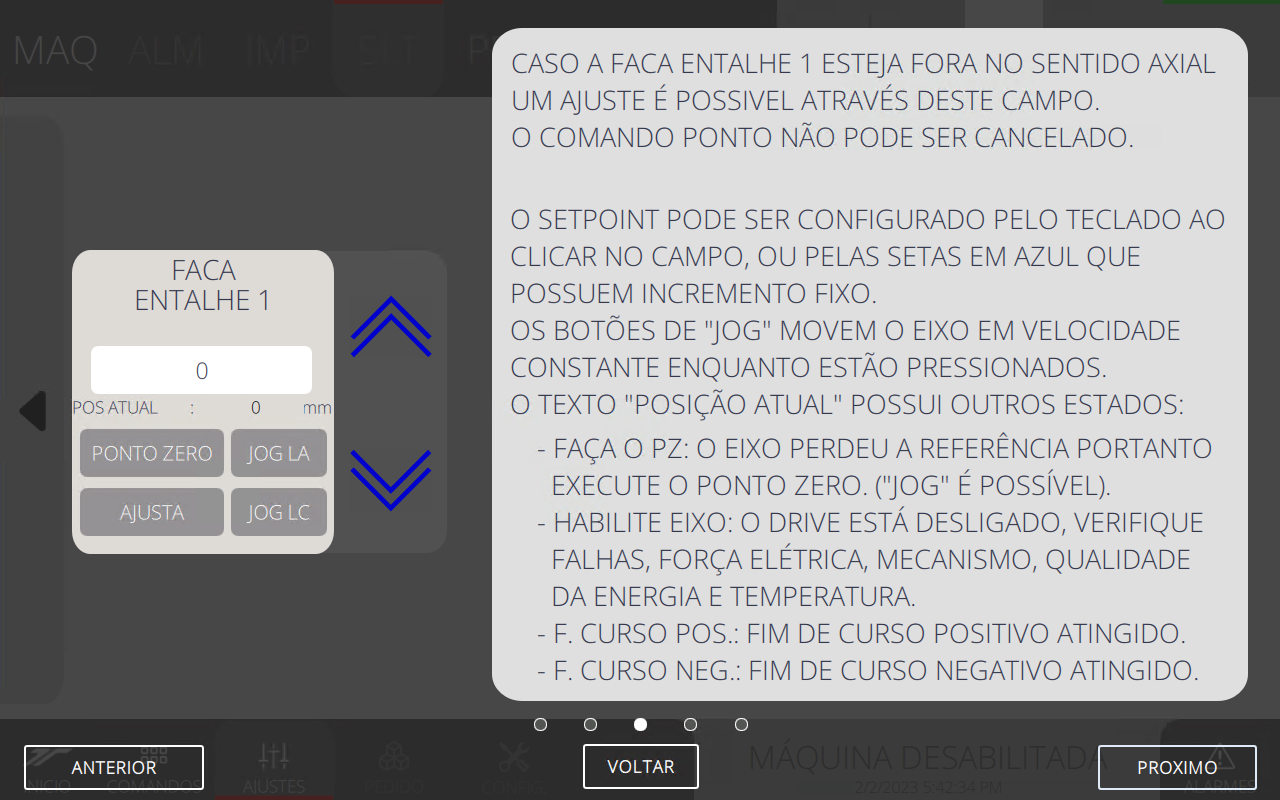
\includegraphics[width=576px,height=360px]{src/imagesFlexo/05-slotter/settings/e-9.png}
\end{figure}
\vspace*{\fill}

\newpage
\thispagestyle{fancy}
\vspace*{40 pt}
\subsubsection{\small{Ajuste da posição axial da faca ENTALHE 3}}\label{telaAjustesSlotterAjusteDaPosicaoAxialDaFacaEntalhe3}
\vspace*{\fill}
\begin{figure}[h]
  \centering
  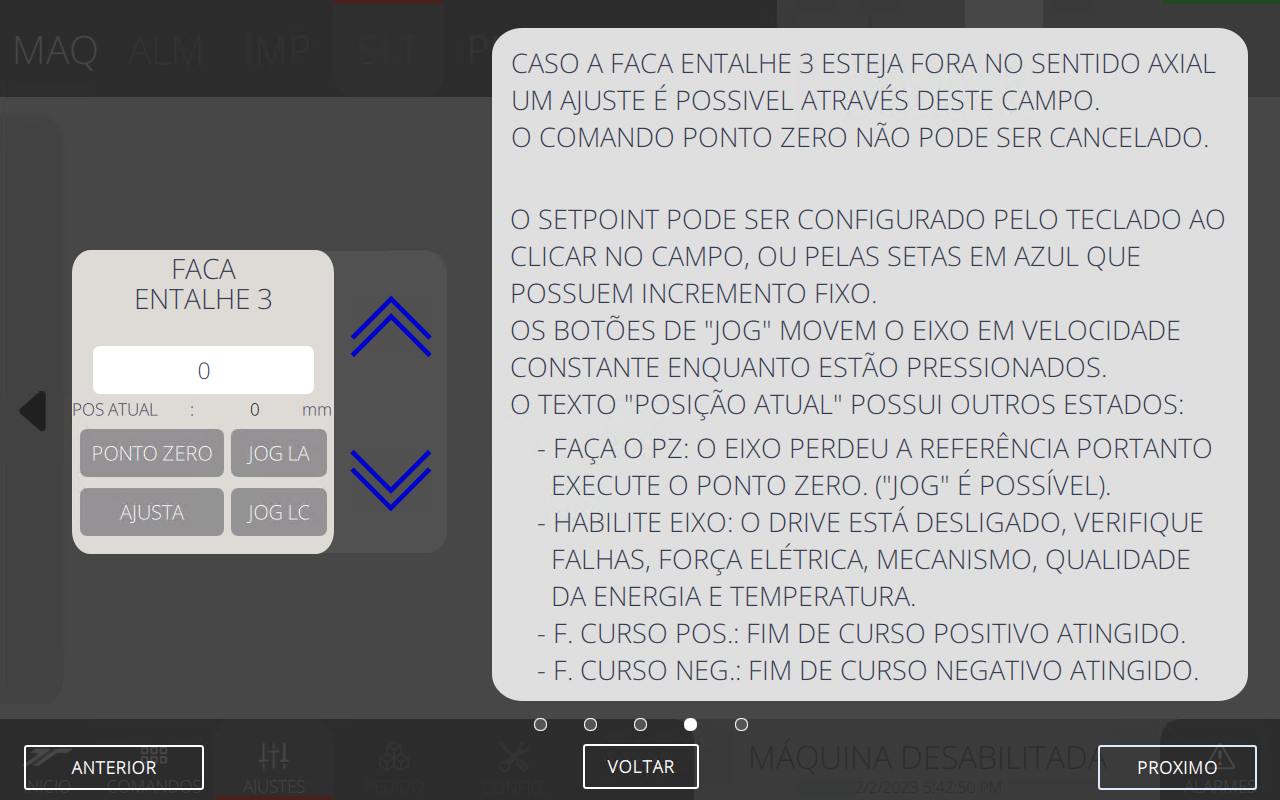
\includegraphics[width=576px,height=360px]{src/imagesFlexo/05-slotter/settings/e-10.png}
\end{figure}
\vspace*{\fill}

\newpage
\thispagestyle{fancy}
\vspace*{40 pt}
\subsubsection{\small{Ajustar a posição axial da faca ENTALHE Refile}}\label{telaAjustesSlotterAjustarAPosicaoAxialDaFacaEntalheRefile}
\vspace*{\fill}
\begin{figure}[h]
  \centering
  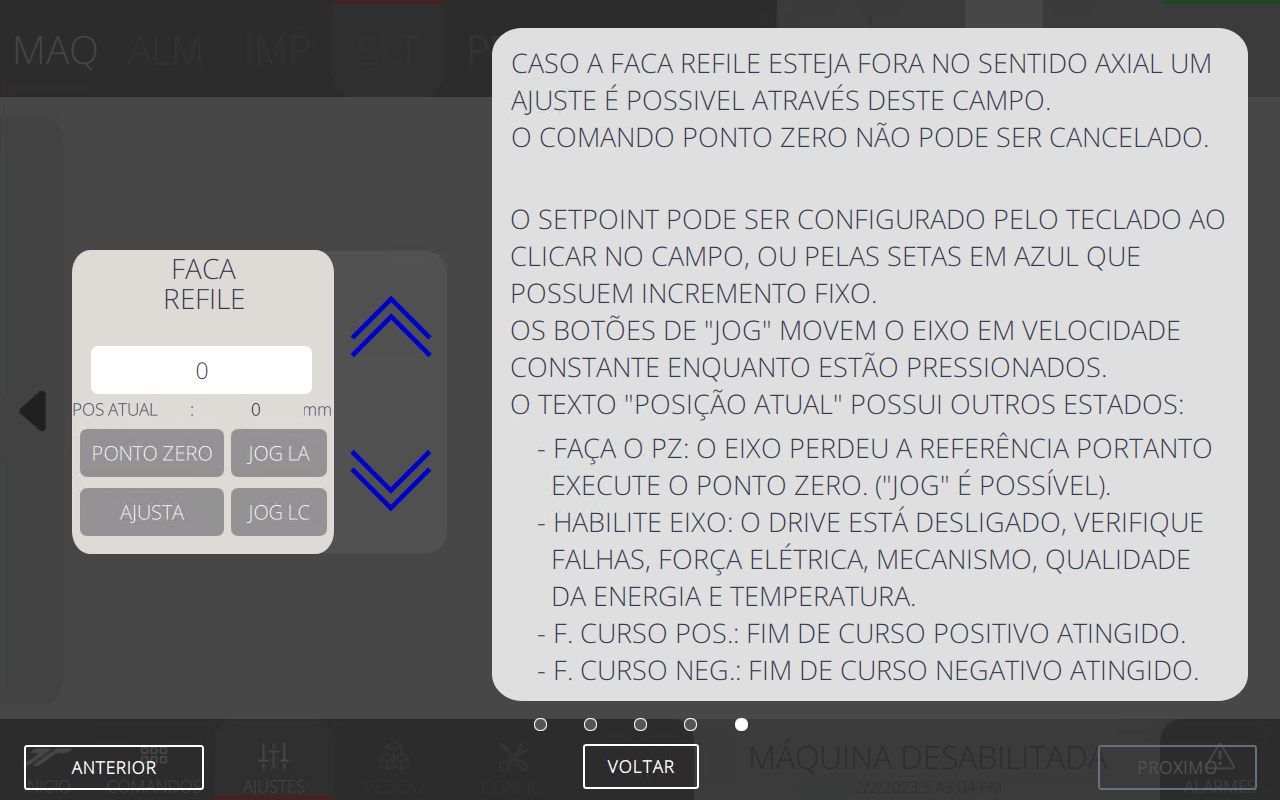
\includegraphics[width=576px,height=360px]{src/imagesFlexo/05-slotter/settings/e-11.png}
\end{figure}
\vspace*{\fill}